\documentclass[twocolumn]{jarticle}

%Confirmation Number: 	226
%Submission Passcode: 	226X-C6J8D6B5B7

\renewcommand{\baselinestretch}{0.75}
\usepackage{NLP}
\usepackage[dvipdfmx]{graphicx}

\title{\textbf{テキストマイニングシンポジウムでの発表内容と言語処理技術}}

\author{
\begin{tabular}{p{8em}p{7em}p{7em}p{8em}}
%\begin{tabular}{llll}
竹内 孔一$^{1}$ &  金山 博$^{2}$ & 市瀬 眞$^{3}$ & 榊 剛史$^{4}$   \\
岡山大学大学院 & 日本アイ・ビー・エム株式会社 東京基礎研究所 & 株式会社NTTドコモ 情報システム部 & 株式会社ホットリンク \\
\vspace{-4ex}
\end{tabular} \and
\begin{tabular}{p{7em}p{8em}p{8em}}
 渡辺 靖彦$^{5}$ &  東中竜一郎$^{6}$ & 嶋田 和孝$^{7}$   \\
 龍谷大学 理工学部& 日本電信電話株式会社 NTTメディアインテリジェンス研究所 & 九州工業大学 大学院情報工学研究院 \\
\end{tabular} 
}
\vspace{-4ex}
\date{\texttt{$^{1}$koichi@cl.cs.okayama-u.ac.jp,
$^{2}$hkana@jp.ibm.com, 
$^{3}$ichisem@nttdocomo.com,
$^{4}$t.sakaki@hottolink.co.jp,
$^{5}$watanabe@rins.ryukoku.ac.jp,
$^{6}$higashinaka.ryuichiro@lab.ntt.co.jp,
$^{7}$shimada@pluto.ai.kyutech.ac.jp}
}

\begin{document}
\maketitle


\section{はじめに} 
電子情報通信学会 言語理解とコミュニケーション研究会
\footnote{http://www.ieice.org/\~{}nlc/}では,
2011年からテキストマイニング・
シンポジウムを開催しており,2016年2月で8回を数えた.これは学術界からの
研究成果と,産業界での実践的な知見に基づく技術や,実務に使う側の知見や
要望を合わせて議論する場として定着してきている.本稿では,過去5年のシン
ポジウムの発表から,学術側から見て特徴的なものを取り上げ,議論されてき
たテーマ,提案された技術,未解決の課題などについて論じたい.また事例を
取り上げた後,テキストマイニング全てに共通した言語処理の置かれている位
置付けを確認し,実社会の要求に応える言語処理の可能性について議論する.



%全てを紹介しきれないが,コールセンター,事故事例,医療,旅行情報,金融情報,経営情
%報といったテキストが対象となり,こうした広範な分野に対して,それぞれに
%特徴の異なる手法が提案されて状況を報告する.これにより言語処理の実応用
%研究の可能性について議論する.



\section{テキストマイニングの目的と基本的な課題}
テキストマイニングには,第2回シンポジウムの那須川氏の講演
\cite{nasukawa2012}にあるように,「大量のテキストデータから役立つ知見を
得る」,より具体的には「個々のテキストの情報だけからは得られない知見を
得る」\cite{nasukawa2012}という目的があると考えられる.また筆者が考える
テキストマイニングの特徴は,この目的を達成する状況として「何を取りだし
て良いか分からない」という状況からスタートすることがあり,検索のタスクでは
本質的に解決できない点である.例えば企業のコールセンターに蓄積されたテ
キストの中で,何が問題になっているかは,キーワードを集約するだけでは把
握することが難しいが,人手で個々のテキストを全て読んで整理することもま
た量的に不可能である.
文献\cite{nasukawa2012}が指摘するように,クラスタリングで抽象化すると意
図が不明になってしまい,文字面ベースだと表現の異なりで分散してしまう.
取り出したい情報が不明な場合,異なる表現を同一視するための辞書を予め作
成することは人手でも不可能である.
これに対して\cite{nasukawa2012}では,単語より長い単位(X がV できない)
での表現の集約を行いつつ,あらゆる語(または商品名など分野に特化した語句)
またはフレーズなどと数値的な比較をすることで実際に有益な知見を得る方法
を実践している(例えば文献\cite{takeuchi2008}).この状況から,
テキストマイニングという研究分野に下記の2点の特徴を見いだせる.

\begin{description}
\item[1] 主眼は有益な知見(とそのエビデンス)の獲得であり,ツールではない
\item[2] 知見を得るためには,ツールを用いて操作する作業者の知識も求められる
\end{description}

従って,言語処理技術の精度の改善が,テキストマイニングの効果に直接的に反映されるとは限らないというのが現実である.
しかし,分野依存辞書の構築\cite{nasukawa04}など共通の課題は存在するのも確かである.
以下,実データに対してどのような要求があるか,どのような分析が行われてきたかを提示することで,現実のタスクに直結するような新たな言語処理研究の課題の創出に貢献したい.


\section{テキストマイニング・シンポジウムで発表された内容}
シンポジウムでは学術的な発表,企業デモ,討論などさまざまな発表スタイルを設けている.
その中で本稿では学術的な要素を含みつつ,現実の問題に対して研究を行っている例
を紹介する.これによってどんな課題でどういう情報を取り出す必要があるか,
また取り出したものが社会的にどういう価値があったかを示すことで
実社会に必要とされる言語処理への事例を提示したい.
%テキストから取りたいものが,定義がかなり難しく,パターン化が絶望的で有り,
%そのなかで,手法として確立すべき要素を提供できるのではと考えられるためである.

{\bf 1) 企業の業績・活動に対するテキストマイニング}\\
記事やSNSから企業活動について企業情報を収集して有益な情報を獲得しようとする
研究報告が10件以上報告されている.その中で経済動向や株価推定の研究が
発表されている.和泉ら\cite{izumi2011}は日本銀行の金融経済月報を利用して,
月ごとの{\bf 単語の主成分スコアの時系列}を特徴として,{\bf 回帰分析}を当てはめることにより
翌月の日本国債市場の運用をテスト評価として行った.その結果,テキストを利用した
ときの方が他の数値を利用した予測より高い利益を得ることを実験的に示した.

羽室ら\cite{hamuro2011}は投資家が近年の配信される金融関係の評判テキストに左右されて
いるかどうか分析するために,Bloomberg社の記事に含まれる評判情報(「需要が伸びる」や
「株価が反発する」など)が株価変動にどのように影響を与えているかを分析している.
ここで企業の評判情報を獲得するための評価表現辞書の構築のために,
{\bf 那須川ら\cite{nasukawa04}の極性辞書構築手法}を利用している.これにより「景気が回復する」という
格助詞と用言のペアによる辞書を構築している.評価表現辞書を利用して,記事から
センチメント指数を求め,株価との相関を調べたところ高い相関があることを示した.
また,シミュレーションによる運用実験でセンチメント指数を入れた場合に実用的に
有効であることを示した.

薄井ら\cite{usui2014}も企業活動ニュースにおける評判評価情報に着目したが,
さらに表現を細分類してニュースのセンチメント値を求める手法を提案している.
まず評価辞書の構築としてニュース記事に対して形態素を{\bf tf-idf}により重み付けして
重要語のみを抽出する(これをキーワードと呼ぶ).次に,各キーワードの極性については
キーワードを含むニュースが配信されたとき,株価が上昇したか下降したかで極性を判定し,
{\bf 重回帰分析}を用いて評価値を付与する.
この方法により例えば「業務改善命令」や「下方修正」など企業活動の
評価に必要な語が獲得できている.これを高村らが作成した極性辞書\cite{takamura05}
と比較したところ,高村らの辞書はこれらのうちの2.6\%程度しか網羅していないことが
わかった.このキーワードベースの評価辞書を用いて,ニュース記事の極性を判定する.
その際,単にキーワードを含む場合の文と,「売り上げ減少に伴い,赤字に転落した」
といった原因-結果を含む評価文を別に評価した.これは因果関係は
株価の影響に対して大きいと考えられるためニュース評価の際により大きな重み
を与えるためである.こうして作成したニュース記事センチメント分析手法を1000文の
ニュース記事と配信後の株価の値動きで評価したところ,プラス評価に対して7割の一致率,
マイナス評価に対して4割の一致率を得たことを示している.精度としてはまだ低いが,
ニュース配信後の株価をテキストに対する評価として利用している部分が興味深い.

廣川\cite{hirokawa2013}らは医薬品製造業68社を対象に有価証券報告書
のテキストから特徴語を抽出し,単語ベクトルに基づくSVMを適用することで,
当該期の企業の利益伸び率が上位α位に入ってるかどうかを判定する手法を提
案した.これらテキストを利用した企業活動推定のポイントは株価や利益率な
ど測定できる数値が存在し,なおかつ発行時期が明確な文書が存在することに
ある.よってこうした良質なデータが存在すれば企業活動の予測が可能である
ことがうかがえる.

一方,こうした評価値との結びつきとは異なる研究も報告されている.
杉原ら\cite{sugihara2012}は営業支援システムに蓄積される営業日報テキストデータから課題記述文を取り出し,
顧客との商談の可能性を広げる取り組みを行っている.課題記述文とは「望ましくない
状況や望ましいゴールといった解決・改善の対象や結果として記述される文」であり,
改善策や問題点が記述されている文である.例えば「人力作業が多く,それに伴う
工数やミスを減らしたい」といった文を取り出す.{\bf SVMによる抽出モデル}を仮定し,
特徴量として課題文に現れやすい,トラブルや要求,解法や評価表現を取り出すための
単語を指定するために{\bf 言語資源}を利用する\footnote{日本語評価極性辞書
(http://www.cl.ecei.tohoku.ac.jp/
index.php?Open~Resources\slash{}Japanese Sentiment
 Polarity Dictionary),
および「負担・トラブル表現リスト」(https://alaginrc.nict.go.jp/)}.
さらに,文書内での文の位置などの文の特徴,自立語n-gram,極性語とPMI値の高い語の頻度数
を特徴量とした.その結果F値で40\%程度の精度を得たことを報告している.
%また坂地,中山,西沢は企業活動の指標を取り出すことで,
%情報集約を行うなどしている.
また酒井\cite{sakai2014}らは企業活動と就職活動時のキーワードがマッチしていないことに
気づき,企業の業績発表記事から活動を表す適切なキーワードを抽出する手法を提案している.

これら上記の研究はいずれもテキストから抽出すべきものが比較的明確である
ため情報抽出に近いタスクと考えられる.一方で,大森\cite{ohmori2013}は数
年にわたる電機業界の活動に対して成長要因を分析するテキストマイニングの
結果を報告している.この際,知識の構造化手法を取り入れた独自の分析フレー
ムワークを仮定し,テキストから得られた{\bf 単語共起グラフ}の解釈から,テキス
トと企業活動の指標を参考に,成長している企業とそうでない企業との差につ
いて海外との標準化や研究への投資があることを明らかにした.
こうした数値指標とテキストを元にした要因分析は分析者の知識構造に頼る
部分が多く,自動化できる部分がほとんどないことがこの研究から
分かる{\footnote{この研究は言語理解とコミュニケーション研究会2013年研究賞を受賞.}.

{\bf 2) 医療・介護・福祉関連}\\
医療や介護に関する発表が数件あり,実務的な課題を明らかにしている.
山下ら\cite{yamashita2014}は病院における手術後の在院日数に着目して,
長期在院者の特徴を推定する研究を提案した.
診療データなどのテキストデータから在院日数
に影響あたえた要因は何かを取り出すのが目的である.手法としては
手術記録文書から医学辞書を利用して重要語を抽出し,{\bf SVM}を利用して
25日以上在院した場合を正例として,正例に寄与した単語を収集するものである.
獲得できた単語が長期滞在にどのように関連していたかはさらなる分析の必要があるが
因子分析の可能性を示した.

大山らは\cite{ohyama2014}介護施設に対してアンケートを行い,
若年性認知症患者の受け入れ拒否理由について得られた自由回答文に対してテキストマイニング
を行った分析を発表している.{\bf 単語間の共起グラフ}から「トラブル」と「暴言」「暴力」 
「ケンカ」との共起が高いことがわかり,実際のアンケート文を確認したところ,
施設側がトラブル発生時の対処に懸念を抱いてることが要因であることを明らかにした.

福田ら\cite{fukuda2014}は介護現場における申し送り情報に対して{\bf 単語間の共起グラフ}
に基づくテキストマイニングを行い,業務改善した実例を複数報告している.1例をあげると,
共起グラフは通常,介助に関する言葉が現れるのに対して,「夫」,
「差し入れ」,「黙る」など異なった共起語が現れた.
これをもとに職員で振り返ったところ,利用者の夫が介護スタッフの見ていないところで
利用者である妻に食事を差し入れていることが判明した.利用者は飲み込みが弱く誤嚥の
可能性があるため,対処として職員のいるところで食事を与えることを認めたところ,
利用者のご家族の満足度が大きく向上した\footnote{この研究は言語理解とコミュニケーション研究会2014年研究賞を受賞.}.

こうした医療まわりの事例からわかることは,人のケアに関わる部分は些細なことでも
当該者にとって重要なできごとであり,個別の対応が求められることが想像される.
よって抽象化や数値化が役に立つ見通しがみえない.つまりテキストの内容がケアの
向上に対して重要な基本データと考えられる.現段階では単語の共起グラフから読み取る
以上の手法が見受けられないが,テキストマイニングが活用されるべき課題と考えられる.


{\bf 3) 政策にかかわる意見集約}\\
葦原ら\cite{ashihara2012}は地方の議会議事録から政策として
求められている要望・要件を取り出す手法を提案している.議会議事録は通常のテキスト
と異なり,議員の質問と回答など,会話になっていること,また,一文が長く並列構造
が多用されるなどの特徴がある.そこで{\bf CBAP\cite{maruyama2003}を利用した文節単位での処理}を提案し,
要求を表す末尾表現である「べき」がどの文節にまで影響するか,議事録を分析して
特徴量とした.要求部分の抽出には{\bf SVM}を利用し,ベースライン(Cabocha+日本語
機能表現辞書)に対してF値で4ポイント以上高いことを示した.

また岩見ら\cite{iwami2016}はエネルギー政策に関するパブリックコメント9万件を
可視化した結果について報告した.手法としては意見を人手により特徴的であると考えられる
クラスに分類し,特徴クラス間の{\bf ネットワークグラフ}を描画して意見の構造化を試みた.
しかしながらネットワーク構造が複雑で有り,ネットワークから全体的な構造をどう
理解するかについては明確な結論は得られなかった.

このように政策に関する意見収集は表現の自由度が高く,数値化の見込みも低いため
テキスト表現が主となるが,単純な評価文ではないため明確な分析手法が見えていない
状況である.既存の係り受け解析だけでなく,文節単位の処理など,長い文に対する
処理を強化した言語処理システムが求められる.

{\bf 4) その他}\\
上記のような大きなテーマの他に高齢者が空いた時間に個人のスキルを活かして
働けるようにするスキルマッチング手法\cite{miura2015}や,
テキスト記事から未来予測部分を取り出すことで
未来予想を取り出す手法\cite{shimaoka2015},陸上競技におけるライバルの
活動状況を獲得してモチベーションを向上する手法\cite{sano2016}など
具体的でテキストに埋もれている有益な情報を利用しようとするアイデアに
あふれた研究が提案されている.
テキストから価値ある情報を取り出す分野が広く,またテキストが同じ性質でないため
各問題に応じた言語処理ツールが求められる.


\begin{figure}[t]
\begin{center}
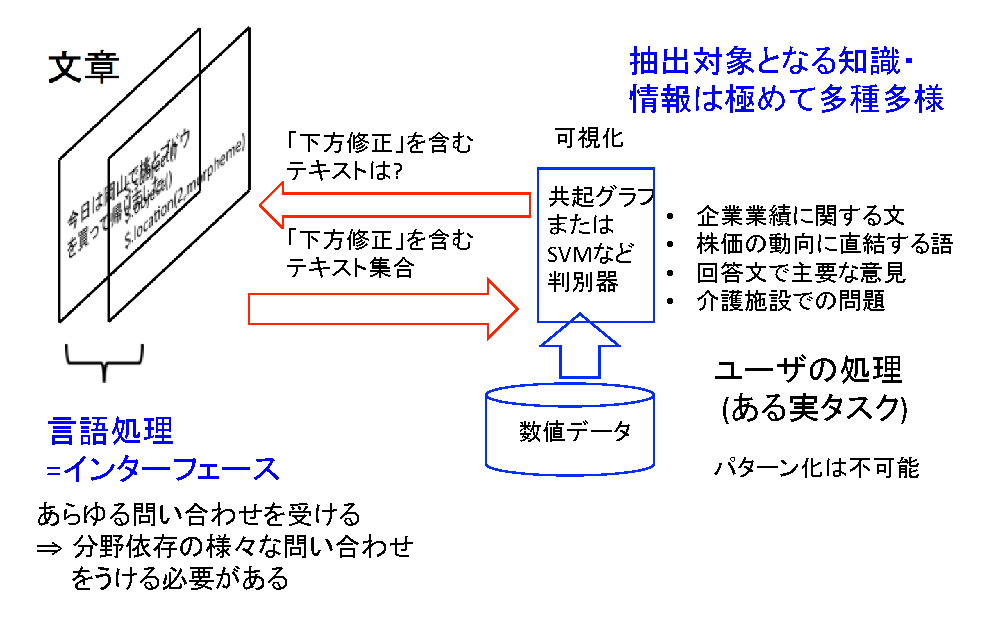
\includegraphics[scale=0.5]{fig/lang.eps}
\end{center}
\caption {言語処理は文書に対するあらゆる問い合わせを受けるインターフェース}
\label{fig:interface}
\end{figure}


\section{言語処理の位置付けと発展}

上記で取り上げたテキストマイニングに関する研究で利用された言語処理や手
法など太字でマークした.その結果,テキストを特定のキーワード(極性辞書や
分野依存の表現) の共起グラフがよく使われていることがわかる.また評価値
(株価などの評価指標)がある場合はSVMが使われている(この場合はキーワード
は特徴量として利用される).
どちらの場合も,"テキストに対する操作"としての言語処理を考えると
キーワードマッチングが主であり,キーワード単独の頻度や共起頻度などを
ある限られたフィルタ(名詞のみなど)で獲得する操作が中心となる.
形態素解析も係り受け解析も,キーワードが目的とする使われ方をしているか
どうかを指定するためのパターンを記述するために利用される.

これは例えばテキストから取り出したい内容が企業情報であれば,
「企業活動を表す文書」を集める必要があり,文の中では「企業名」
やその「活動」を表現する部分を獲得し,表現の正規化が必要になる.しかし直接
こうした文を獲得するツールは存在しないため,「企業活動を表す文書」を表すには,
そうした記事を書いているニュースサイトを固定したり,「活動」などはキーワードを
決めるか「動詞」といった品詞レベルで押さえるといった手法しかない.

つまりテキストから必要な情報を取り出す状況において,分野非依存のツールだけでは
解決せず,問題・分野に依存したテキスト情報抽出手法を分析者側が構築できないため
キーワードベースでの方法で代替している状況であると考えられる.
この状況を図\ref{fig:interface}に示した.よって言語処理はテキストに対して
あらゆる要求に対して情報を獲得できるツールを構築していく必要があるのでは無いか
と考えられる.テキストマイニングの主は価値ある情報であり,分析者はツール構築に興味は無い.
この部分において,言語処理を研究している研究者が分析者と共同で活動することで
より具体的な実処理に役立つ研究テーマと成果が得られるのではないかと推察できる.


\bibliographystyle{jplain}
\bibliography{ws2016}
\end{document} 

